\documentclass{standalone}
\usepackage{tikz}
\begin{document}
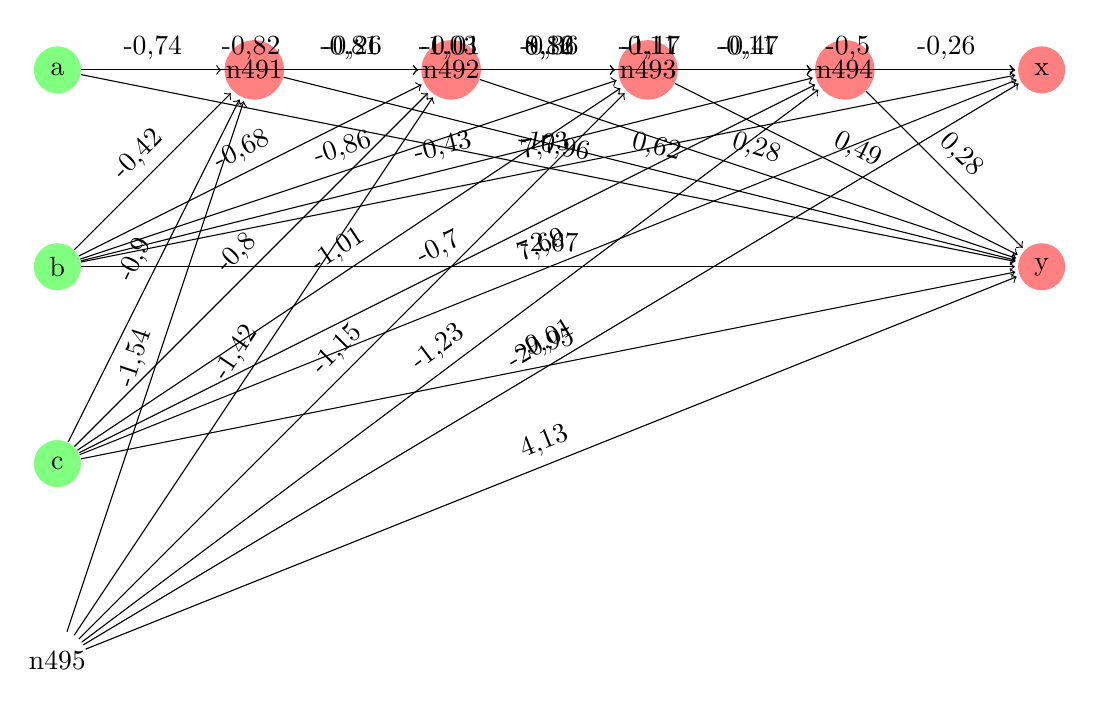
\begin{tikzpicture}[shorten >=1pt,->,draw=black!,node distance=2.5cm]
\tikzstyle{neuron}=[circle,fill=black!25,minimum size=17pt,inner sep=0pt]
\tikzstyle{constant}=[neuron, fill=white!50];
\tikzstyle{sigmoid}=[neuron, fill=red!50];
\tikzstyle{identity}=[neuron, fill=green!50];
\node [identity] (a) {a};
\node [identity,below of=a] (b) {b};
\node [identity,below of=b] (c) {c};
\node [constant,below of=c] (n495) {n495};
\node [sigmoid,right of=a] (n491) {n491};
\node [sigmoid,right of=n491] (n492) {n492};
\node [sigmoid,right of=n492] (n493) {n493};
\node [sigmoid,right of=n493] (n494) {n494};
\node [sigmoid,right of=n494] (x) {x};
\node [sigmoid,below of=x] (y) {y};
\path[every node/.style={sloped,anchor=south,auto=false}]
(n492) edge node {0,28} (y)
(n492) edge node {-0,47} (x)
(n492) edge node {-0,11} (n494)
(n492) edge node {0,16} (n493)
(n491) edge node {-1,17} (x)
(n491) edge node {0,62} (y)
(n491) edge node {-0,01} (n493)
(n491) edge node {-0,26} (n492)
(n491) edge node {-0,36} (n494)
(n494) edge node {0,28} (y)
(n494) edge node {-0,26} (x)
(n493) edge node {-0,5} (x)
(n493) edge node {0,49} (y)
(n493) edge node {-0,11} (n494)
(n495) edge node {4,13} (y)
(n495) edge node {-1,54} (n491)
(n495) edge node {-20,01} (x)
(n495) edge node {-1,23} (n494)
(n495) edge node {-1,42} (n492)
(n495) edge node {-1,15} (n493)
(b) edge node {-2,67} (y)
(b) edge node {7,73} (x)
(b) edge node {-0,68} (n492)
(b) edge node {-0,42} (n491)
(b) edge node {-0,43} (n494)
(b) edge node {-0,86} (n493)
(a) edge node {8,82} (x)
(a) edge node {-1,03} (n494)
(a) edge node {-0,74} (n491)
(a) edge node {-10,96} (y)
(a) edge node {-0,81} (n493)
(a) edge node {-0,82} (n492)
(c) edge node {7,69} (x)
(c) edge node {-0,9} (n491)
(c) edge node {-9,95} (y)
(c) edge node {-1,01} (n493)
(c) edge node {-0,8} (n492)
(c) edge node {-0,7} (n494)
;\end{tikzpicture}
\end{document}